\chapter{Sortierverfahren}

\section{Lösungsvorschlag}

\subsection{Aufgabenteil a)}

\begin{itemize}
    \item Es gilt, dass jedes allgemeine Sortierverfahren mindestens $\Omega(n\ log\ n)$ Schlüsselvergleiche benötigt (vgl.~\cite[154]{OW17b}).\\
    Diese untere Schranke gilt sowohl für die \textit{elementaren Sortierverfahren}\footnote{s. ~\cite[81]{OW17b}}  (\textbf{Insertion}-,
    \textbf{Selection}- und \textbf{Bubble}-Sort), die im \textbf{worst-case} $O(n^2)$ Zeit benötigen, als auch für die
    Verfahren, die eine \textbf{divide and conquer}-Strategie implementieren, wie \textbf{Quicksort} ($O(n^2)$)
    und \textbf{Merge-Sort} ($O(n\ log\ n)$ ).

    \item Bei sehr wenigen Datensätzen (in der Aufgabe mit $n \leq 100$ angegeben) ist die Wahl des Sortierverfahren
    hinsichtlich Effizienz im Sinne von Speicherplatzverbrauch als auch der benötigten Laufzeit eher nebensächlich, wenn man davon ausgeht,
    dass das Sortieren auf einem der heutigen Technik entsprechenden Rechner mit einem der o.a. Verfahren durchgeführt wird.\\
    Qualitätskriterien wie Einfachheit der Implementierung und Verständlichkeit können hier eher ins Gewicht gefallen (vgl. \cite[5 f.]{GD18a}).

    \item Andere Kriterien, die die Eingabedaten betreffen, können jedoch die Auswahl des Sortierverfahrens beeinflussen: Sind die Daten überwiegend
    vorsortiert, kann bspw. \textbf{Insertion-Sort} verwendet werden, das bei vorsortierten Daten lineare Laufzeit erreichen kann (vgl. \cite[188]{CL22})\footnote{
        \textit{Ottmann und Widmayer} führen außerdem \textbf{Smoothsort} von Dijkstra an, dass $O(n)$ für eine vorsortierte Folge und $O(n\ log\ n)$ benötigt (vgl.~\cite[112]{OW17b})
        }.

    \item Bei kleinen Problemgrößen fällt genau die damit verbundene Anzahl der Eingabedaten $n$ stärker ins Gewicht.
    Benötigt bspw. eine Implementierung von Insertion-Sort $8*n^2$ Schritte und eine Implementierung von Merge-Sort $64*n\ log\ n$ Schritte, so ist
    Insertion Sort für $n \leq 43$ effizienter als Merge-Sort (s. Abbildung~\ref{fig:insertionvsmerge})\footnote{
    \textit{Cormen et. al.} empfehlen einen \textit{Hybrid} aus Merge-Sort und Insertion-Sort in \cite[45, Problem 2-1]{CL22}, worauf auch \textit{Sedgewick und Wane} in \cite[275]{SW11} hinweisen.
    } \footnote{
        bei einem direkten Vergleich von Merge-Sort und Bubble-Sort dürfte schnell klar werden, dass ein unsortiertes Feld mit $n=2$ von Bubble-Sort mit weniger Operationen sortiert wird, als das bei Merge-Sort der Fall ist, wo neben dem Sortieren und Verschmelzen der Eingabefolgen außerdem zusätzlich linear viel Speicher für die Teilfolgen benötigt wird.
    }.

    \item In der Literatur finden sich Empfehlungen für Quick-Sort, das für typische Eingabedaten im Durchschnitt $O(n\ log\ n)$ Zeit benötigt und in-place arbeitet (vgl. \cite[182 ff.]{CL22}).

    \item Für eine hohe Zahl von Datensätzen, die auch im \textbf{worst-case} optimale Laufzeit aufweist, kann \etxtbf{Merge-Sort} verwendet werden, das mit $O(n\ log\ n)$ \textit{worst-case-optimal} ist (vgl.\cite[116]{OW17b}).
\end{itemize}


\begin{figure}
    \begin{center}
        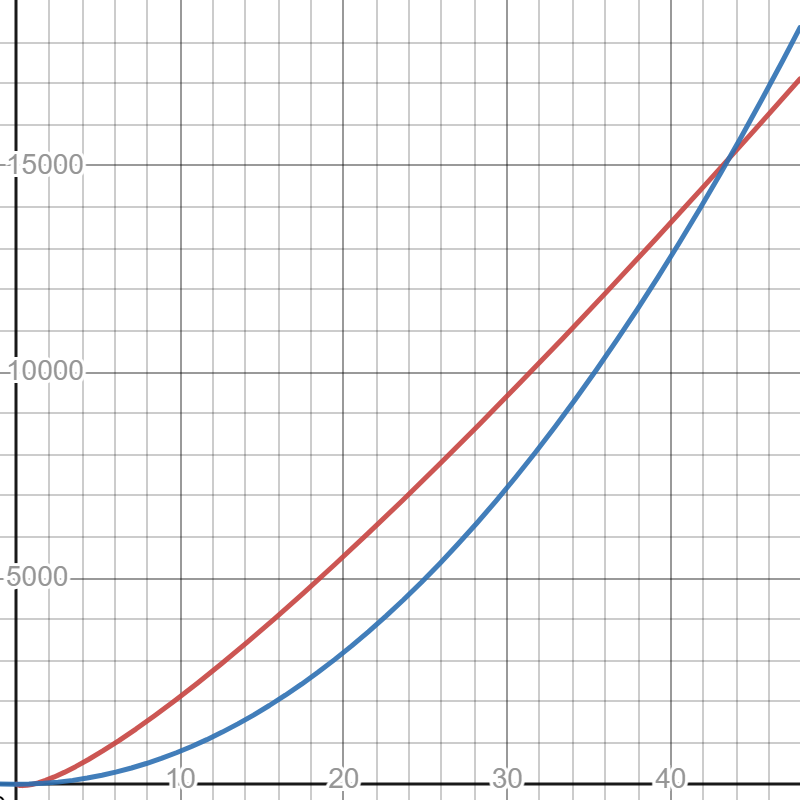
\includegraphics[scale=0.3]{chapters/7. Sortierverfahren/img/insertionvsmerge}
        \caption{Für eine Eingabelänge von $n\leq43$ arbeitet eine Implementierung von Insertion-Sort, die im Beispiel $8*n^2$ Schritte (blau) benötigt, effizienter als eine Implementierung von Merge-Sort, die im Beispiel $64*n*log\ n$ Schritte (rot) benötigt. (Quelle: eigene)}
        \label{fig:insertionvsmerge}
    \end{center}
\end{figure}

\subsection{Aufgabenteil b)}

Bei dem vorgestellten Sortierverfahren handelt es sich um \textbf{Selection-Sort}.
Bei dem Sortierverfahren wird ein Feld $A$ mit einer Problemgröße $n$ und einem geg. Index $i$ mit $ 0 \leq i \leq n - 2$ Teilfolgen $[A_{i+1}, ... , A_n]$ nach einem kleinsten Schlüssel $A_{min} < A_{i}$ durchsucht, wobei $A_{min}$ in der jeweiligen Teilfolge auch der kleinste Schlüssel ist.\\
Der gefundene Schlüssel wird dann mit $A_i$ getauscht.\\
Die Teilfolgen enthalten so jeweils einen kleinsten, dann den zweitkleinsten, dann den drittkleinsten, ... , und schließlich den größten Schlüssel, die Vertauschung ergibt dann zum Schluss ein aufsteigend sortiertes Feld (s. \cite[82]{OW17b}).


\subsection{Aufgabenteil c)}

Die Laufzeit eines Algorithmus ist die Summe der Laufzeiten jeder einzelnen ausgeführten Anweisung.\\
Eine Anweisung, die aus insg. $c_k$ (Elementar-)Operationen besteht, und die $m$-mal aufgerufen wird, trägt zu der Laufzeit mit $c_k * m$ bei (vgl.~\cite[29 f.]{CL22}).\\

\noindent
Im Folgenden werden die Kosten für die Aufrufe von Zeile 5 berechnet, aus denen der Wert von \code{vergleich} abgeleitet werden kann:

\begin{minted}[mathescape,
    linenos,
    baselinestretch=1.75,
    numbersep=5pt,
    gobble=2]{java}
    while (i < arr.length - 1) {                    // $c_1$   $n$
        min = arr[i];                               // $c_2$   $n-1$
        minIndex = i;                               // $c_3$   $n-1$
        for (int j = i + 1; j < arr.length; j++) {  // $c_4$   $\sum_{i=0}^{n-2}t_i$
            vergleiche++;                           // $c_5$   $\sum_{i=0}^{n-2}(t_i - 1)$
            if (arr[j] < min) {                     // $c_5$   $\sum_{i=0}^{n-2}(t_i - 1)$
                minIndex = j;                       // $c_7$   $\sum_{i=0}^{n-2}(t_i - 1)$
                min = arr[j];                       // $c_8$   $\sum_{i=0}^{n-2}(t_i - 1)$
            }
        }
        arr[minIndex] = arr[i];                     // $c_9$   $n-1$
        arr[i] = min;                               // $c_{10}$   $n-1$
        i++;                                        // $c_{11}$   $n-1$
    }
\end{minted}\\

\noindent
Für $i = 0, 1, 2, .. n - 2$ ist $t_i$ die Anzahl der Aufrufe der Schleifenbedingung in Zeile $5$.\\
Wie schon an der Gesamtlaufzeit für Zeile 1 und Zeile 2 ersichtlich, wird eine Schleifenbedingung immer ein mal mehr aufgerufen, als das davon abhängige Statement (der \textit{Block} in unserem Fall\footnote{s. ``14.12. The while Statement``: \url{https://docs.oracle.com/javase/specs/jls/se21/html/jls-14.html#jls-14.12} - abgerufen 19.2.2024
}).\\

\noindent
Für Zeile 1 des o.a. Listings ergeben sich mit $i = 0$ und $n=arr.length$ somit $n-1$ Aufrufe\footnote{
Ergibt der Ausdruck in der Schleifenbedingung \code{false}, ist das Feld entweder leer ($n=0$) oder es gilt $i < n - 1$.
Wir gehen im folgenden von $n > 0$ aus.
}.\\
Das nachfolgende Statement der while-Schleife\footnote{
    s. ``14.12. The while Statement``: \url{https://docs.oracle.com/javase/specs/jls/se21/html/jls-14.html#jls-14.12} - abgerufen 19.2.2024
} (in Form eines \textit{Blocks} in Zeile 2-13) wird $n-2$-mal aufgerufen.\\
Der Block der \code{for}-Schleife (Zeile 5-9) wird in Abhängigkeit von $i$ aufgerufen: Für $i = 0$ wird er $n - 1$ mal aufgerufen, für $i = 1$ $n - 2$-mal usw.\\

\noindent
Für die Zählvariable $j$ gilt

\begin{equation}
j := n \in \mathbb{N},  j \geq i+1, j \leq n-1
\end{equation}

\noindent
Für die Anzahl der Aufrufe der Schleifenbedingung $t_i$ gilt\footnote{Endwert der Summe ist $n$, da die Schleifenbedingung ein mal mehr als der nachfolgende Block aufgerufen wird}:

\begin{equation}
    t_i = \sum_{j=i+1}^{n} 1
\end{equation}

\noindent
Die Kosten $T(n_4)$ für Zeile 4 lassen sich somit wie folgt berechnen:

\begin{equation}
    T(n_4) = c_4 * \sum_{i=0}^{n-2} t_i = c_4 * \sum_{i=0}^{n-2} \sum_{j = i + 1}^{n} 1
\end{equation}

\noindent
Die Summe lässt sich weiter auflösen zu

\begin{equation}
\begin{split}
    \sum_{i=0}^{n-2} \sum_{j = i + 1}^{n} 1 &= \sum_{i=0}^{n-2} \sum_{j = 1}^{n-i} 1\\
    &= \sum_{i=0}^{n-2} (n - i)\\
    &= \sum_{i=1}^{n-1} (n - (i - 1)) \\
    &= \sum_{i=1}^{n-1} n - \sum_{i=1}^{n-1} (i + 1)\\
    &= n * (n - 1) - \frac{n * (n - 1)}{2} + n - 1\\
    &= \frac{n * (n + 1)}{2} - 1
\end{split}
\end{equation}


\noindent
wodurch sich letztendlich die Kosten berechnen lassen mit

\begin{equation}
    T(n_4) = c_4 * (\frac{n * (n + 1)}{2} - 1)
\end{equation}

\noindent
Die Anzahl der Aufrufe von $c_4$ ist dann $m_{c_4} = \frac{n * (n + 1)}{2} - 1$


\noindent
Jeder Aufruf von $c_5$ findet aufgrund des Abbruchs der Schleife\footnote{
    Überprüfung der Schleifenbedingung $j < arr.length$
} $t_i - 1$-mal statt.\\
Für die Gesamtzahl der Aufrufe $m_{c_5}$ von $c5$ muss deshalb $n-1$ von $m_{c_4}$ subtrahiert werden:

\begin{equation}
    m_{c5} = (\frac{n * (n + 1)}{2} - 1) - (n-1)) = \frac{n * (n - 1)}{2}
\end{equation}

\noindent
was der Anzahl der Aufrufe von Zeile 5 entspricht, und somit zu dem Wert von \code{vergleiche} führt\footnote{
    entsprechend führt das Skript (Teil 2) auf Seite 160 die Anzahl an Vergleichen auf.
}.